\namedchapter{Technologieauswertung}{J} \label{chap:Technologieauswertung}
Im Kapitel der Technologieauswertung untersuchen wir Programmiersprachen, Frameworks, Datenbanktechnologien und weitere Bibliotheken hinsichtlich ihrer Eignung für unsere gewählte Architektur-Option. Alle Abschnitte bis auf den letzten befolgen hierbei einen ähnlichen Aufbau. Zunächst werden die Kriterien aufgeführt, dann der Vergleich ausgeführt und zum Schluss folgt eine Auswertung und Diskussion der Ergebnisse.

\namedsection{Programmiersprachen}{J}
Allein der Vergleich zwischen zwei Programmiersprachen könnte vermutlich einen ganzen Bericht füllen. Gerade deshalb sollte es klar umrissene Kriterien geben die bei der Gewichtung helfen. Diese werden bereits zu beginn ausführlich diskutiert.
Im nächsten Abschnitt werden mehrere Programmiersprachen auf Grundlage unserer zuvor diskutierten Kriterien verglichen und eingeordnet.
Zuguterletzt werden die Ergebnisse der Evaluierung tabellarisch zusammengefasst und kritisch hinterfragt.

\subsection{Evaluierungskriterien}
Für jedes Kriterium werden wir kurz beschreiben was es bedeutet und anschließend ausführen warum es für unser Projekt von Bedeutung ist.
\begin{description}
    \item [Performanz]
    Wie schlägt sich die Programmiersprache hinsichtlich Speicherverbrauch, CPU-Auslastung und Request-Durchsatz?
    Wenn die Sprache einen geringeren Speicherverbrauch aufweist, kann die Chunk-Größe für die Batchjobs vergrößert und dadurch die Zeit bis zur Abarbeitung verkürzt werden.
    Wenn der Request-Durchsatz hoch ist, können mehr Anfragen pro Zeiteinheit bewältigt werden was der Skalierbarkeit zugute kommt.
    \item [Verbosität]
    Wie effizient ist die Sprache hinsichtlich ihrer Syntax? Lässt sich mit wenig Code bereits viel bewältigen? Wie schnell lassen sich mit der Sprache Resultate erzielen?
    Wenn es sich mit einer Sprache besonders produktiv arbeiten lässt können bessere Resultate in gleicher Zeit erzielen.
    \item [Ökosystem]
    Wie groß ist die Community? Wie gut lassen sich weitere Bibliotheken und Dokumentationen finden?
    Umso mehr Informationen frei zur Verfügung stehen desto schneller kann man eventuelle Probleme aus dem Weg räumen oder sich in Sprachkonzepte einarbeiten (z.B. Multithreading).
    \item [Erfahrungen]
    Wie viel Vorwissen besitzen die Teammitglieder mit der Programmiersprache?
    Bereits vorhandenes Wissen nutzen um effizienter zu einer Lösung kommen zu können.
    \item [Sonstiges]
    Was sind weitere erwähnenswerte Eigenschaften der Sprache oder Bestandteile des Ökosystems?
    Es könnte bereits Clients für Drittsysteme geben oder einige Eigenschaften der Sprachen kommen unserer Architektur besonders entgegen.
\end{description}

\subsection{Betrachtete Programmiersprachen}
Die Wahl der untersuchten Programmiersprachen hängt auch mit der Wahl der untersuchten Frameworks zusammen. Insofern werden in diesem Abschnitt die Programmiersprachen Java, C\#, JavaScript (und TypeScript), PHP sowie Python betrachtet.

Um die Informationen aus den Tabellen \ref{tab:comp_pl1} und \ref{tab:comp_pl2} besser einordnen zu können folgt eine kurze Erläuterung zu den wichtigsten Spalten und Quellen. In vielen Fällen ergeben sich die endgültigen Ergebnisse aus der Aggregation aller Daten der Quellen.

Mit Request-Durchsatz ist in der Regel die Anzahl der bearbeiteten Anfragen pro Zeiteinheit bei gleichwertiger Hardware gemeint. In den aufgeführten Quellen wurde dies auf unterschiedliche Weise probiert. Entweder mit Server die direkt ohne weitere Operation antworten oder die Aufgaben mit typischen Arbeiten im Lebenszyklus eines Servers emulieren.

Die CPU-Performanz bezieht sich auf die Laufzeit und Auslastung von Arbeitseinheiten für unterschiedliche Programmiersprachen. Eine Programmiersprache die effizienter arbeitet indem sie die Aufgabe in kürzerer Zeit abarbeitet oder CPU-Kerne besser auslastet wird demzufolge besser bewertet. Für diesen Punkt wurde vornehmlich das Benchmarks Game betrachtet und alle Werte verglichen.

Die Spalte mit der Bezeichnung "Umfang Third-Party" enthält gesicherte Angaben über die Anzahl einzigartiger Bibliotheken aus den meistgenutzten Third-Party-Datenbanken der jeweiligen Programmiersprache. Erwähnenswert ist in diesem Zusammenhang, dass man die Werte für npm kritisch betrachten sollte, weil JavaScript insbesondere im Frontend-Umfeld genutzt wird. Dadurch hat JavaScript im Vergleich zu anderen auch viel mehr grafische Komponenten als Bibliotheken. Darüber hinaus gibt es keine zuverlässige Auskunft über die Qualität einzelner Bibliotheken in den jeweiligen Third-Party-Datenbanken.

Der Punkt Community wertet vor allem diverse Ranglisten zur Popularität der Sprachen aus. Unser Ansatz ist die Überlegung, dass eine höhere Popularität auch mit mehr hilfreiche Quellen für die Programmiersprachen einhergehen. In der Regel greifen diese Ranglisten in vielen Fällen auf Informationen wie Anzahl der Ergebnissen aus Suchmaschinen zurück. Für präzisere Informationen wurde auch auf Daten von Stackoverflow und Github zurückgegriffen.

\begin{table}[H]
    \centering
    \begin{tabular}{|p{3cm}|p{5cm}|p{5cm}|}
    \hline
    \textbf{Programmier- sprache}          & \textbf{C\#}                                                                & \textbf{Java}                                                           \\ \hline\hline
    Erschienen                     & 2000                                                               & 1995                                                           \\ \hline
    Programmier- paradigma \cite{wiki_pl}           & vornehmlich objekt-orientiert mit Ausätze für andere Paradigma     & vornehmlich objekt-orientiert mit Ausätze für andere Paradigma \\ \hline
    Statisch / Dynamisch typisiert \cite{wiki_type} & statisch                                                           & statisch                                                       \\ \hline
    Stark / Schwach typisiert \cite{wiki_type}      & stark                                                              & stark                                                          \\ \hline
    Intepretiert                   & ja (Bytcode)                                                       & ja (Bytecode)                                                  \\ \hline
    Speicherverwalt- ung             & Garbage Collector                                                  & Garbage Collector                                              \\ \hline
    Multithreading                 & ja                                                                 & ja                                                             \\ \hline
    Request-Durchsatz \cite{mihai_benchmark,tandemseven_perf,techempower_benchmark,benchmark_web,medium_awslambda,acloud_awslambda}              & gut                                                                & sehr gut                                                       \\ \hline
    CPU-Performanz \cite{benchmark_game,benchmark_kostya}                & sehr gut                                                           & sehr gut                                                       \\ \hline
    Verwendung                     & Enterprise                                                         & Enterprise                                                     \\ \hline
    Erfahrungen                    & wenig                                                              & gut                                                            \\ \hline
    Umfang Third-Party             &  nuget ca. 180k \cite{csharp_packages}                           & gradle/maven ca. 315k \cite{java_packages}         \\ \hline
    Community \cite{stackoverflow_survey,tiobe,pypl,github_octoverse,redmonk}                      & moderat                                                            & sehr gut                                                       \\ \hline
    Anmerkungen                    & Third-Party Bibliotheken häufig kommerziell ausgelegt, Typsystem & OFTP Client/Server Referenzimplmentierung verfügbar, Typsystem \\ \hline
    \end{tabular}
    \caption {Vergleich Programmiersprachen C\# und Java}
    \label{tab:comp_pl1}
\end{table}

\begin{table}[H]
    \centering
    \begin{tabular}{|p{3cm}|p{3.7cm}|p{3.7cm}|p{3.7cm}|}
    \hline
    \textbf{Programmier-sprache}                                                                        & \textbf{JavaScript (Node.js)}                                                              & \textbf{Python}                                                  & \textbf{PHP}                                                                                                \\ \hline\hline
    Erschienen                                                                                   & 1995 (2009)                                                                        & 1990                                                    & 1995                                                                                               \\ \hline
    Programmier- paradigma \cite{wiki_pl} & ursprünglich prozedural, mittlerweile Ausätze für andere Paradigma, keine Generics & vornehmlich prozedural mit Ausätze für andere Paradigma & vornehmlich objekt-orientiert mit Ausätze für andere Paradigma, keine Generics, nicht event-driven \\ \hline
    Statisch / Dynamisch typisiert \cite{wiki_type}                                                              & dynamisch                                                                          & dynamisch                                               & dynamisch                                                                                          \\ \hline
    Stark / Schwach typisiert \cite{wiki_type}                                                                   & schwach                                                                            & stark                                                   & schwach                                                                                            \\ \hline
    Intepretiert                                                                                 & ja                                                                                 & ja                                                      & ja                                                                                                 \\ \hline
    Speicherverwalt -ung                                                                        & Garbage Collector                                                                  & Garbage Collector                                       & Garbage Collector                                                                                  \\ \hline
    Multithreading                                                                               & ja                                                                                 & ja                                                      & ja                                                                                                 \\ \hline
    Request-Durchsatz \cite{mihai_benchmark,tandemseven_perf,techempower_benchmark,benchmark_web,medium_awslambda,acloud_awslambda}                                                                           & I/O intensiv sehr gut \cite{performance_io}                                                              & moderat                                                 & gut                                                                                                \\ \hline
    CPU-Performanz \cite{benchmark_game,benchmark_kostya}                                                                               & gut                                                                                & moderat                                                 & moderat                                                                                            \\ \hline
    Verwendung                                                                        & Frontend, API                                                                      & Datenanalyse, Machinelles Lernen, Automatisierung     & Web Backend, API                                                                                   \\ \hline
    Erfahrungen                                                                                  & gut                                                                                & wenig                                                   & wenig                                                                                              \\ \hline
    Umfang Third-Party                                                                           & npm über 1 Million \cite{js_packages}                                    & pip pypi ca. 210k \cite{python_packages}              & composer packagist ca. 250k \cite{php_packages}                                \\ \hline
    Community \cite{stackoverflow_survey,tiobe,pypl,github_octoverse,redmonk}                                                                                    & sehr gut                                                                           & sehr gut                                                & gut                                                                                                \\ \hline
    Anmerkungen                                                                                  & JSON ist Bestandteil der Sprache                                                 & ~                                                       & ~                                                                                                  \\ \hline
    \end{tabular}
    \caption {Vergleich Programmiersprachen JavaScript, Python und PHP}
    \label{tab:comp_pl2}
\end{table}

Nun zurück zur eigentlichen Gegenüberstellung. Grundsätzlich haben Java und C\# aufgrund ihrer Beschaffenheit hinsichtlich dem vorherigen kompilieren zum Bytecode und dem Ansatz bzgl. der dynamischen und starken Typisierung einen Performance-Vorteil. Dieser spiegelt sich, wie bereits zuvor erwähnt, auch in einigen Benchmarks wieder. Jedoch fehlt für C\# den meisten Teammitgliedern an Erfahrung und auch das Ökosystem ist im Vergleich zu Java bedeutend kleiner, sodass auch das einarbeiten aufwändiger wäre.

Demgegenüber könnte man Java und JavaScript (bzw. TypeScript) stellen, welche ein ähnlich starkes Ökosystem bieten und bei denen auch die Vorerfahrungen im Team ähnlich sind. Allerdings kann JavaScript längst nicht so stark in Punkto Typesicherheit, Multithreading und CPU-Effizienz auftrumpfen. Zusätzlich bietet Java den Vorteil, dass es z.B. für QDX eine Referenzimplementierung gibt.

Man könnte vielleicht noch argumentieren, dass Python im Bezug auf Verbosität einen Vorteil für die Produktivität haben könnte \cite{expressiveness}. Dem kann man gegenüberstellen, dass durch Frameworks wie Spring Boot und Bibliotheken wie Project Lombok die Verbosität bei Java geradezu minimal ist. Mehr Informationen darüber gibt es im Abschnitt \ref{sec:libraries}.

\subsection{Auswertung und Diskussion}

Insgesamt lässt sich also zusammenfassen, dass Java für uns die beste Wahl ist. In der Tabelle \ref{tab:programming_language_evaluation} können nochmal die einzelnen Kriterien und Bewertungen auf einer Skala von 1 - 5 für jede Programmiersprache eingesehen werden.
\begin{table}[!h]
\centering
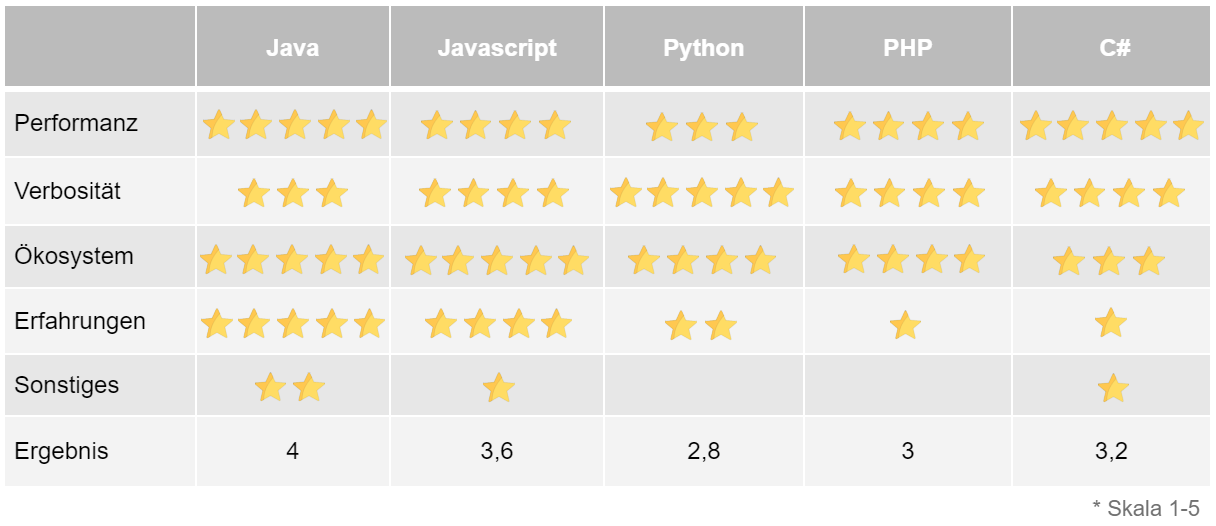
\includegraphics[width=14cm]{images/0x_technology_stack/programming_language_comparison_table.png}
\caption{Auswertung Programmiersprachen.}
\label{tab:programming_language_evaluation}
\small{Sonstiges sind Bonus-Punkte}
\end{table}

Generell hilft es für das Verständnis der Analyse für Programmiersprachen unsere Auswertung im Kontext unserer Architekturwahl zu sehen. Mithin hängt sie inhaltlich auch stark mit der Analyse für die Frameworks zusammen. Viele der hier aufgeführten Ergebnisse werden vermehrt auch in den Abschnitten zu den Frameworks genutzt.

Gerade im Umfeld von Datenintegration ist davon auszugehen das Reserven bei Speicher-Auslastung und die höhere CPU-Effizienz bei Java einen wichtigen Vorteil gegenüber den meisten anderen Sprachen haben.

Ebenfalls nicht unerwähnt bleiben sollte der Umstand bei JavaScript, dass theoretisch auch als Grundlage für die Entwicklung anstatt Node.js auch $\mu$WebSockets (wird unter anderem für Crypto-Handelsplatz Coinbase genutzt) gewählt werden könnte, dass mit einer immensen Performancesteigerung bei den Request-Durchsatz einhergeht. Mit dem Nachteil, dass viele Bibliotheken aus dem JavaScript Ökosystem nicht mehr ohne weiteres genutzt werden können.

\newpage

\namedsection{Frameworks}{J}
Für jedes Problem gibt es das passende Handwerkszeug. Es ist nicht nachhaltig jedes benötigte Versatzstück erneut zu implementieren, wenn es bereits ein passendes dazu gibt. In den folgenden Abschnitten wollen wir demzufolge herausfinden welches Framework unsere Anforderungen an die Architektur, Produktivität und vorhandenen Erfahrungen am Besten abdeckt.

\namedsubsection{Evaluierungskriterien}{J}
Für jedes Kriterium werden wir kurz beschreiben was es bedeutet und anschließend ausführen warum es für unser Projekt von Bedeutung ist.
\begin{description}
    \item [Performanz]
    Wie performant ist die Technologie?
    Wie verhält sich die Technologie bei der Verarbeitung von großen Datensätzen?
    Wie gut ist das Handling für High Throughput von I/O-Aufgaben?
    Wenn der Durchsatz hoch ist, können mehr I/O-Aufgaben pro Zeiteinheit bewältigt werden was der Skalierbarkeit zugute kommt.
    \item [Komplexität]
    Wie komplex ist die dafür benötigte Infrastruktur und Setup?
    Wie groß ist  der Einarbeitungsaufwand in die Technologie?
    Eine Einarbeitung in eine riesige Microservice-Landschaft mit dutzenden Services erfordert mehr Zeit als ein Monolith. Ähnlich verhält es sich mit den Infrastrukturaufwand.
    \item [Dokumentation / Community]
    Wie qualitativ ist die offizielle Dokumentation?
    Wie groß und aktiv ist die Community?
    Wie viel zusätzliches Lernmaterial ist öffentlich verfügbar?
    Bei genügend Beispielen und eine aktive Community verkürzt es die Einarbeitungszeit.
    \item [Team Know-How]
    Wie viel Vorwissen haben die Teammitglieder mit der Technologie?
    Bereits vorhandenes Wissen nutzen um effizienter zu einer Lösung kommen zu können.
    \item [Skalierbarkeit]
    Wie gut lässt sich die Applikation skalieren?
    Wie sehr ist die Technologie für Enterprise-Projekte geeignet?
    Kommt das Framework bereits mit vordefinierten Lösungen für Microservice-Architekturen, dann erleichtert es den Aufbau einer eigenen modularen Softwarearchitektur.
\end{description}

\namedsubsection{Betrachtete Frameworks}{J}
In diesem Bereich untersuchen wir der Reihe nach die Frameworks Spring (Boot), Loopback, Express, Flask, Slim
und .NET. Der Aufbau enthält jeweils eine Beschreibung und spezifische Charakteristika des Frameworks und endet schließlich in einer Zusammenfassung der Vorteile und Nachteile.

\subsubsection*{Spring\hfill[J]}
Spring ist ein modulares, quelloffenes Java-Framework mit dem Ziel, die Entwicklung von Java/Java EE zu vereinfachen und gute Programmierpraktiken zu fördern.

\begin{figure}[!h]
\centering
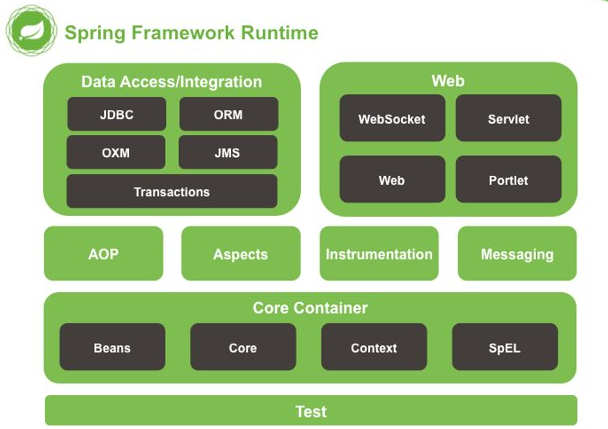
\includegraphics[width=9cm]{images/0x_technology_stack/spring_framework_runtime.png}
\caption{Spring Framework Runtime \cite{springruntime}}
\end{figure}

Spring Boot ist ein Framework zur Entwicklung von allein lauffähigen, für den produktiven Einsatz geeigneten Spring-basierten Applikationen ("convention over configuration") und benötigt keinen Applikationsserver, sondern wird als Fat-Jar-Artefakt inklusive einem eingebetteten Webserver (z.B. Apache Tomcat/Netty) ausgeliefert. Somit wird bereits ein großteil der sonst notwendigen Arbeitsschritte vom Framework selbst übernommen.

Es basiert auf Java ist modular und flexibel aufgebaut. Als Open Source Framework das bereits sehr lange existiert hat es auch eine große Community. Allein das Hauptrepository vereint bereits 20.000 Commits und 414 Contributors auf sich.

\subsubsection*{Vorteile}
\begin{itemize}
    \item Sehr gute Dokumentation und sehr große Community
    \item Umfangreiches Ökosystem mit vielen Libraries
    \item Eignung für CPU-intensive Aufgaben durch Multithreading
    \item Bietet API für Non-blocking I/O für High Throughput Applikationen bei geringer Ressourcennutzung an
    \item JVM ist sicher und hat sich über die Jahre bereits bewährt
    \item Bessere Performance als Skriptsprachen, da der JVM mehrere Metadaten während der Runtime zur Verfügung stehen
    \item Enterprise Support über Pivotal verfügbar
    \item Enterprise Ready Framework
\end{itemize}

\subsubsection*{Nachteile}
\begin{itemize}
    \item Java code ist verbose und es ist viel Boilerplate Code im Vergleich zu anderen Technologien erforderlich
    \item Komplexes Framework, welches Einarbeitung erforderlich macht
\end{itemize}

\subsubsection*{Loopback 4\hfill[J]}
Ein von IBM entwickeltes Enterprise Framework, dass auch in der Cloud gut lauffähig ist. Das Framework ist kompatibel zu Express Middlewares und profitiert so von einem bereits umfangreichen Ökosystem. Versucht zudem durch "Convention over Configuration" den Aufwand bei Entwicklungsarbeiten zu reduzieren.

Grundsätzlich wird TypeScript für das Framework benutzt aber es ist auch möglich darauf zu verzichten und JavaScript zu nutzen. Allerdings wird es nicht empfohlen. Insgesamt ist Loopback 4 wie Spring auch, sehr modular und flexibel aufgebaut. Genauso ist Loopback 4 auch als Open Source Projekt konzipiert ist jedoch bedeutend jünger. Das Hauptrepository umfasst gerade mal 2.900 Commits und 104 Contributors.

\begin{figure}[!h]
\centering
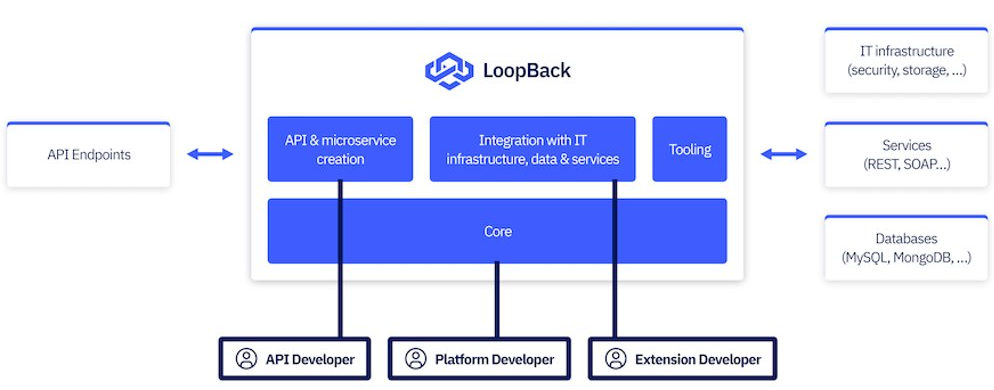
\includegraphics[width=13cm]{images/0x_technology_stack/loopback_4.png}
\caption{Loopback 4 Diagramm \cite{loopback4}}
\end{figure}

\subsubsection*{Vorteile}
\begin{itemize}
    \item Gute Erweiterbarkeit durch Express.js Middlewares
    \item Konnektoren für Datenbankanbindung sind bereits vorhanden
    \item Hohe Modularisierung durch SOA
    \item Weniger Fehleranfällig als reine JavaScript Applikationen, da TypeScript Fehler bereits beim kompilieren abfängt
    \item Schnelle Ergebnisse mit überschaubaren Programmieraufwand
    \item Zugriff auf das größte Package Repository aller Sprache; derzeit über 1 Millionen Packages verfügbar
\end{itemize}

\subsubsection*{Nachteile}
\begin{itemize}
    \item Junges Framework (2018)
    \item Einarbeitung in Framework spezifische Logik notwendig
    \item Performance-Nachteile, da basierend auf High Level Programmiersprache
    \item Relativ kleine Community (2398 commits)
\end{itemize}

\subsubsection*{Express\hfill[Filip]}
Express ist ein minimalistisches open source Webframework für Javascript mit starkem Fokus auf Flexibilität im Ansatz von benutzerdefinierten, im Gegensatz zu standardisierten, bewährten Vorgehensweisen. Es ist Teil des aktuell größten Ökosystem aller Programmiersprachen - Node.js und ist mit über 47.000 Sterne, 5.500 Commits und 230 Contributors in dem Hauptrepository das größte aller in Node.js verfügbaren Webframeworks.

Es basiert auf einer modularen Architektur mit individuellen Funktionalitäten, die als Plugins verfügbar sind. Zu den wichtigsten Merkmalen gehören eine große Auswahl an Template Engines, robustes Routing und hohe I/O-Performanz.

\subsubsection*{Vorteile}
\begin{itemize}
    \item Große Community und gute Dokumentation
    \item Zugriff auf das größte Package Repository aller Sprache; derzeit über 1
Millionen Packages verfügbar
    \item Für das Erstellen von APIs ausgelegt
    \item Gut geeignet für das Handling von High Throughput I/O
    \item Stark reduziertes Boilerplate Code
    \item Einfache Integration von NoSQL-Datenbanken
    \item JSON ist Subset von JavaScript
    \item Kein Kompilierungsschritt notwendig, was zu schnelleren Entwicklungszeiten führt
\end{itemize}

\subsubsection*{Nachteile}
\begin{itemize}
    \item Performance-Verlust, da High-Level Programmiersprache
    \item Für CPU intensive Aufgaben schlecht geeignet
    \item Mehr Runtime Errors sind möglich
\end{itemize}

\subsubsection*{Flask\hfill[Filip]}
Flask ist ein minimalistisches, Python basiertes open source Webframework. Einfachheit, stark reduziertes Boilerplate code und schnelle Entwicklung von Prototypen sind seine wichtigste Merkmale. Sehr hohe Flexibilität und Erweiterbarkeit ist durch Teilung in sehr granulare individuelle Komponente erreicht. Dieser Ansatz resultiert aber in erhöhtem Aufwand – mehr Entscheidungen sind selbst dem Entwickler gelassen.

Das Framework profitiert von einem großem und aktivem Community – das Projekt Repository umfasst gerade mal über 3.800 Commits und über 560 Contributors.

\subsubsection*{Vorteile}
\begin{itemize}
    \item Gute Dokumentation
    \item Für rapid Prototyping geeignet
    \item Schnelle Lernkurve
    \item Leicht erweiterbar
\end{itemize}

\subsubsection*{Nachteile}
\begin{itemize}
    \item Relativ kleine Community
    \item Weniger 'Out of the Box' Funktionalität
    \item Keine gute ORM Mapping Unterstützung
    \item Erbt Python-bezogene Performanzprobleme
\end{itemize}

\subsubsection*{Slim\hfill[Filip]}
Slim ist ein PHP basiertes open source Micro-WebFramework. Es unterstützt alle gemeinsame Szenarien, eignet sich aber besonders gut für APIs Entwicklung und für Rapid Prototyping. Ähnlich zu Python Flask sind bei Slim Einfachheit und Geschwindigkeit der Entwicklung große Vorteile. Die Reichheit an Bibliotheken ist jedoch nicht so groß relativ zu anderen bewerteten Frameworks – für die Projektumsetzung besonders relevant sind die ORM tools die im Slim noch nicht ausgereift sind.

Das Framework verfügt über eine relativ aktive, wenn nicht so große Community. Das Repository fasst aktuell etwa 4.000 Commits von fast 200 Contributors um.
\subsubsection*{Vorteile}
\begin{itemize}
    \item Gute Dokumentation
    \item Für rapid Prototyping geeignet
    \item Einbinden von Drittanbietern über Packagist möglich
    \item Leichte und schnelle Einarbeitung
\end{itemize}

\subsubsection*{Nachteile}
\begin{itemize}
    \item Relativ kleine Community
    \item Keine gute ORM Mapping Unterstützung
    \item ORM Mapping tools nicht komplett ausgereift
\end{itemize}

\subsubsection*{ASP.NET\hfill[Filip]}
ASP.NET ist ein etabliertes, open source, C\# basiertes Framework, das von Microsoft entwickelt wurde und auf der MVC Architektur basiert. Seine wichtigste Designziele sind Skalierbarkeit, Performanz und Sicherheit.

Das Framework profitiert von einer sehr großen und aktiven Community. Das Hauptrepository verfügt aktuell über ca.  Sterne, 40.700 Commits und 670 Contributors.

\begin{figure}[!h]
\centering
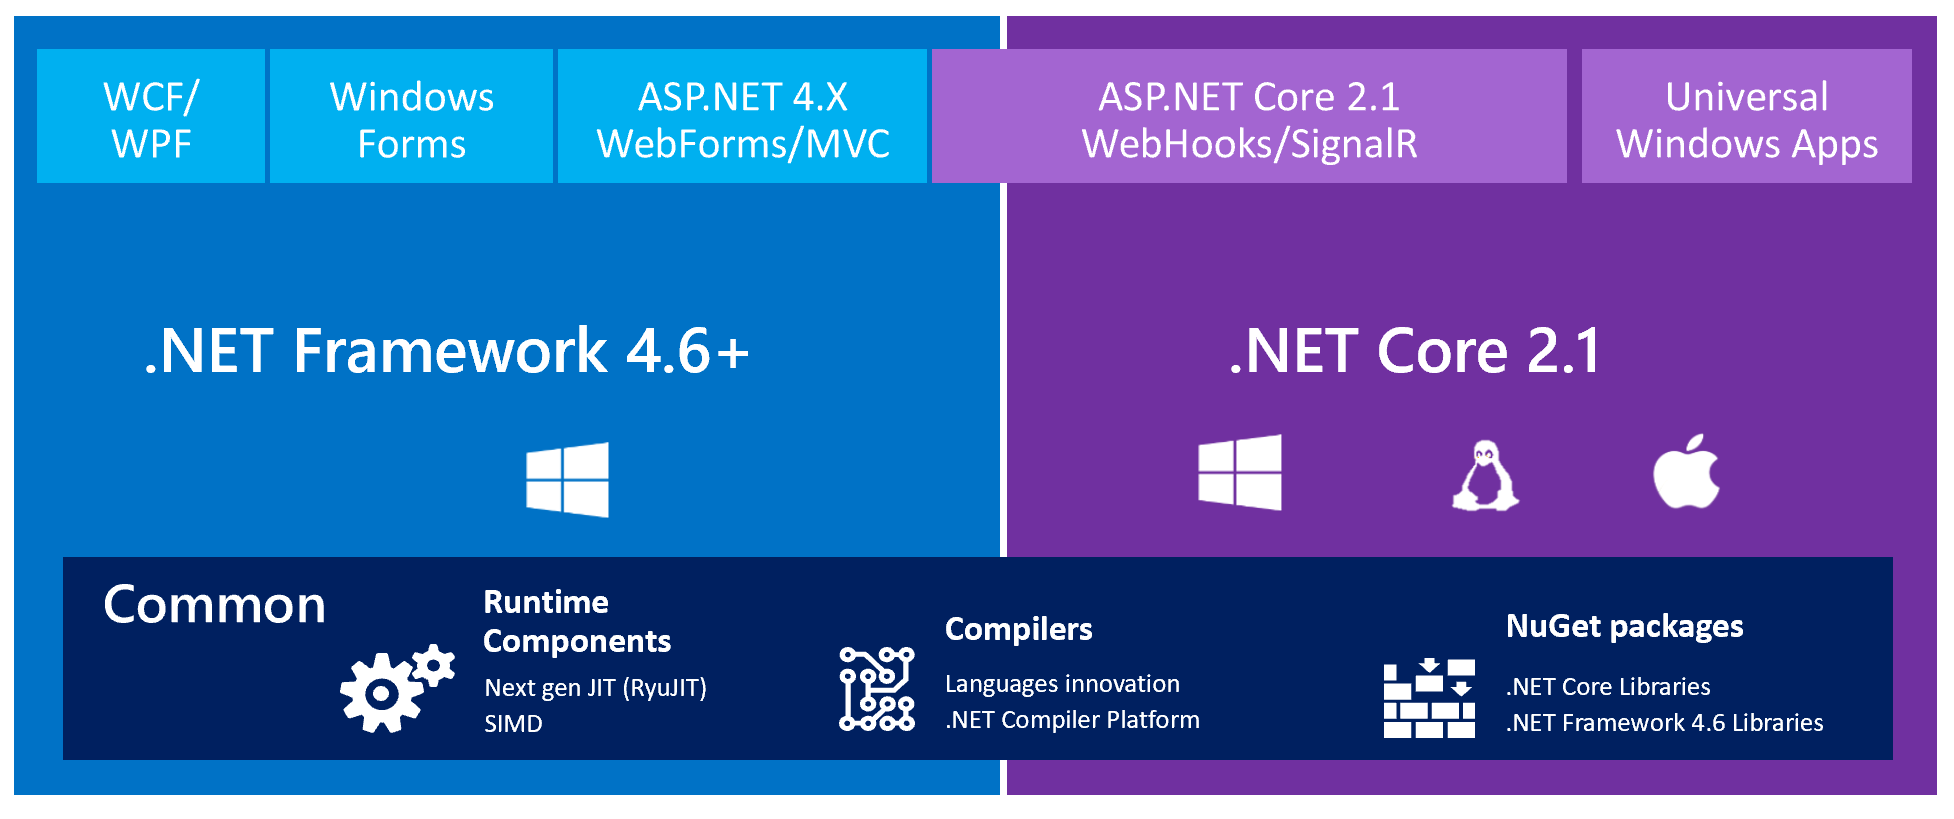
\includegraphics[width=11cm]{images/0x_technology_stack/asp_net.png}
\caption{ASP.NET}
\end{figure}
\subsubsection*{Vorteile}
\begin{itemize}
    \item Sehr große Community und gute Dokumentation
    \item Reiche Funktionalität ohne zusätzlichen Libraries
    \item Einfachere Fehlererkennung und hohe Robustheit wegen starker Typisierung
    \item Enterprise Support vorhanden
\end{itemize}

\subsubsection*{Nachteile}
\begin{itemize}
    \item ORM Mapping nicht flexibel genug
    \item Viele Libraries sind komerziell
\end{itemize}

\namedsubsection{Auswertung und Diskussion}{J}
Aus der Tabelle \ref{fig:framework_evaluation} kann unsere Auswertung entnommen werden. Die Zuteilung der Sterne hat sich aus der Gewichtung der Vor- und Nachteile der jeweiligen Frameworks ergeben. In den folgenden Absätzen werden wir einen Überblick auf hoher Ebene geben. Ziel war es die wichtigsten Gründe für oder gegen einzelne untersuchte Frameworks benannt zu haben.

Spring Boot bewährt sich seit Jahrzehnten im Enterprise-Umfeld. Es bietet reichlich getestete Komponenten zur Erweiterung inklusive Security. Darüber hinaus existiert hier die meiste Erfahrung im Team und eine umfangreiche Dokumentation mit zahlreichen Beispielen und Bootstrap-Projekten. Zudem ist Java bei der Performance für CPU-intensiven Aufgaben, zusammen mit C\#, am stärksten. Direkte Datenbankverbindungen ist ebenfalls ein starker Bereich in Java. JDBC schlägt teilweise sogar ODBC, das in C geschrieben ist.

\begin{table}[]
\centering
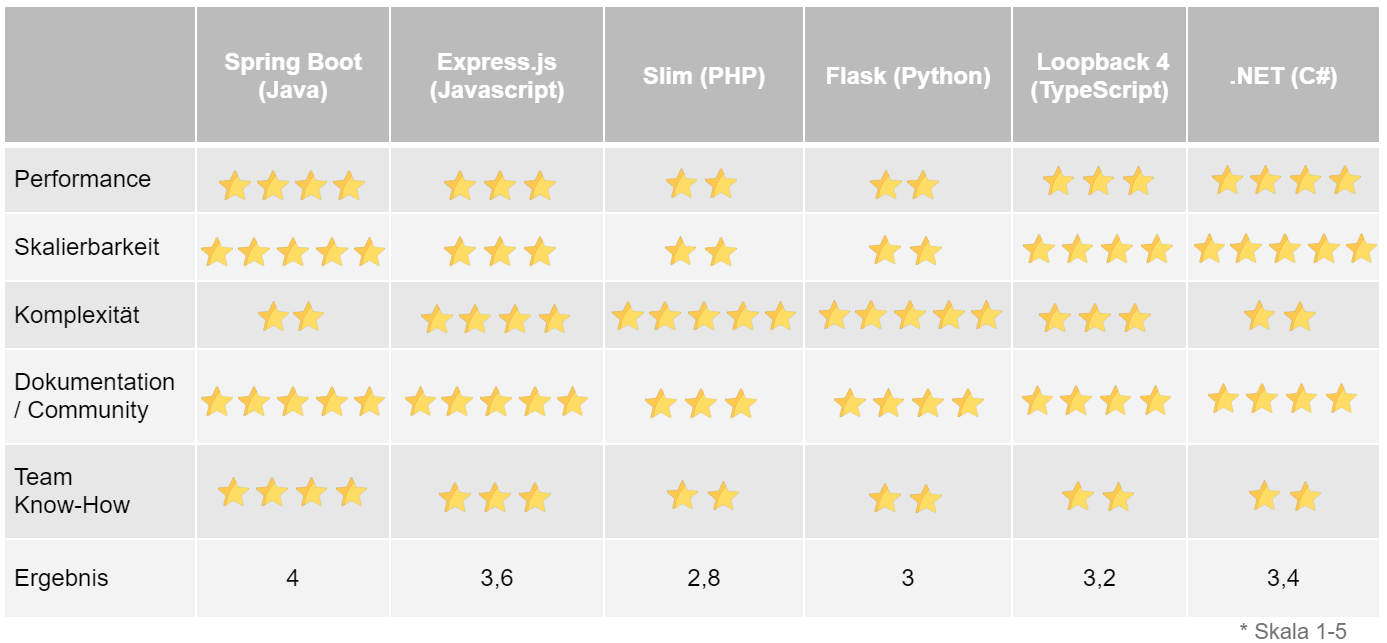
\includegraphics[width=16cm]{images/0x_technology_stack/frameworks_comparision_table.png}
\caption{Framework Auswertung}
\label{fig:framework_evaluation}
\end{table}

Express.js, Slim und Flask sind mehr wie Microframeworks die vor allem das Grundgerüst für das Entwickeln von APIs bereitstellen. Dazu gehört unter anderem das Routing und Middlewares. Demnach müssen einige Bestandteile entweder über Packages bezogen, falls überhaupt vorhanden, oder selbst programmiert werden.

Loopback 4 bietet zwar viele Bausteine an, die für eine Datenintegration relevant sind, allerdings ist das Projekt noch ziemlich jung (2018). Ferner hat es speziell im CPU-lastigen Bereich das Nachsehen im Vergleich zu Java wie aus dem Abschnitt zu den Programmiersprachen zu entnehmen ist.

Alles rund um das .NET Ökosystem ist insbesondere aufgrund der kaum vorhandenen Erfahrungen im Team nicht relevant für uns.

\newpage

\namedsection{Datenbanktechnologien}{Filip}
Persistente Speicherung der Daten ist ein der zentralen Elementen jeder Softwareanwendung. Verschiedene Technologien legen Fokus auf unterschiedliche Aspekte der Speicherung, Abruf und Anfragen. Die dadurch resultierende Trade-offs erzwingen eine genauere Analyse der unterschiedlichen Ansätze um die optimale Technologie für den Use-Case zu wählen.

\subsection{Evaluierungskriterien}
Im Folgenden werden Bewertungskriterien definiert und erläutert, anhand derer die beiden Datenbankarchitekturen verglichen und bewertet werden. Nach der Evaluierung wird diejenige Technologie ausgewählt, die den Projektzielen am besten entspricht.

\begin{description}
    \item [Schema]
    Wie sieht die Struktur für die  Datensätze aus? Welche Eigenschaften hat sie? Wie flexible ist sie?
    \item [Format]
    In welchem Format sind die Daten gespeichert? Sind unterschiedliche Formate erlaubt? Wie werden die Relationen/Abhängigkeiten zwischen Datensätze abgebildet?
    \item [Querying]
    Wie komplex können die Anfragen an Datenbank sein? Wie effizient werden sie verarbeitet?
    \item [BASE Compliance]
    Folgt die Datenbank die ACID (Atomicity, Consistency, Integrity, Durability)oder eher BASE (Basic Availability, Soft state, Eventual consistency) Prinzipien?
\end{description}
\subsection{Betrachtete Datenbanktechnologien}
\subsection*{\textbf{Relationale Datenbanken (RDBMS)}}
Relationale Datenbanken basieren auf einem feststehenden Schema in Form von einer relationalen Tabelle. Als die Spalten den Attributen entsprechen, ist jede Zeile ein Datensatz, jedes optionale Attribut ist also auch in dem Datensatz enthalten. Die Abhängigkeiten zwischen Daten können durch 1:1, 1:m und n:m Relationen zwischen Tabellen realisiert werden. 

Das einheitliche Schema und tabellenbasierte Organisierung der Daten ermöglicht effiziente und komplexe Anfragen über Daten aus mehreren Tabellen mit ausgebauten Kriterien und Bedingungen. Sowohl die Anfragen an die Daten als auch Definitionen der Tabellen, Attributen und Relationen sind in SQL geschrieben.

Relationale Datenbanken folgen die ACID Prinzipien. Eine Reihe von Operationen ist ACID konform, wenn die als eine Einheit betrachtet werden kann (Atomicity), nach der Ausführung die Datenbank in einen validen Zustand bringt (Consistency), gleichzeitig mit anderen solchen Einheiten bearbeitet werden kann (Isolation) und wenn ausgeführt und abgeschlossen dauerhaft wirkt unabhängig von eventuellen Systemausfälle.

\subsection*{\textbf{Nicht-relationale Datenbanken (Non-RDBMS)}}
Nicht-relationale Datenbanken haben im Gegensatz zu RDBMS kein festes Schema und verzichten auf das rigide tabellenbasierte Organisierung der Datensätze. Stattdessen werden die Einträge in Form von Objekte, Dokumente, Schlüssel-Wert Paare oder auch Graphen gespeichert. Die Daten innerhalb einer Sammlung können unterschiedliche Attribute und Struktur haben. 

So großer Freiheitsgrad bei der Struktur und Format wirkt aber negativ die Möglichkeiten, an das System Anfragen zu stellen. Die konkrete Funktionalität hängt von der konkreter Art und Implementierung der Datenbank, ist aber im Allgemeinen weniger mächtig.

Nicht-relationale Datenbanken folgen im Allgemeinen die BASE Prinzipien. Hier sind die Regeln weniger strikt als bei ACID mit dem Ziel, unter anderem bessere Skalierbarkeit und
Elastizität zu erreichen. Somit garantiert die Base Availability, dass die Datenbank die meiste Zeit verfügbar ist. Soft state bedeutet, dass die verschiedene Kopien der Daten nicht immer alle gleichzeitig konsistent sein müssen. Letztlich sorgt Eventual Consistency dafür, dass die Änderungen in endlicher Zeit an alle Kopien angewendet werden und somit alle Kopien den konsistenten Zustand erreichen.

\subsection{Auswertung und Diskussion}
Das umzusetzende Projekt hat unter anderem Anpassbarkeit und Erweiterbarkeit als wichtige Anforderungen, die besser von den nicht relationalen Datenbanken erfüllt sind. Non-RDBMS skalieren besser mit dem wachsenden Dataset. Sie sind auch besser geeignet für Cloud-Speicher und rapide, agile Entwicklung, wo sich die Details der Struktur bzw. des Formats der Daten öfter ändern können. Weiterhin sind für den zu entwickelnden Use-Case die komplexen Abfragemöglichkeiten nicht relevant, da die Daten vorher bereits transformiert worden sind. Auch hohe Verfügbarkeit über die Zeit ist viel wichtiger als die von ACID garantierte absolute Konsistenz. Somit stellt sich eine nicht relationale Art der Datenbank als die am besten geeignete Datenbanktechnologie fest.

Ein weiterer Punkt, der Diskussion noch vorliegt, ist die konkrete Art des Non-RDBMS. Man hat hier Auswahl zwischen vielen verschiedenen Varianten, wobei Schlüssel-Wert basierte, Graphenbasierte und Dokumentenbasierte die drei meist etabliert sind. Eine Schlüssel-Wert basierte Datenbank bietet sehr schnelle Lese- und Schreiboperationen an, die Struktur und Eigenschaften der Werte sind jedoch unübersichtlich. Der graphenbasierter Ansatz ist nur bei starker Vernetzung der Daten vorteilhaft und fokussiert mehr auf der Relationen zwischen Datensätzen als auf den Datensätzen selbst. Die dokumentenbasierte Variante ist Erweiterung des Schlüssel-Wert-Models auf strukturiertes Format. Es ermöglicht verschiedene Formate innerhalb einer Sammlung und eignet sich am besten für die Arbeit mit großen Datenmengen deren Struktur nicht unbedingt gleich bleibt.
\newpage

\namedsection{Weitere Bibliotheken}{J}
\label{sec:libraries}
Dieser Abschnitt beschreibt Bibliotheken die in unserem Projekt zur Anwendung gekommen sind. Generell sollte man sich den Ablauf für das Beziehen von Daten vergegenwärtigen. Zunächst können Drittsystem auf unterschiedlichen Wegen angesprochen werden. Das kann auf Protokollebene sein wie SOAP, REST oder QDX aber auch im Bezug auf die Beschaffenheit der Daten. Diese müssen in den meisten Fällen auf unsere definierten Domänenmodelle angepasst werden. Erst dann können die Daten schlussendlich in unsere Datenbank zwischengespeichert werden. Die meisten der aufgeführten Bibliotheken helfen uns genau für diesen Fall weiter.

\subsection*{Project Lombok}
Eine immense Arbeitserleichterung verschafft uns der Annotation-Processor Project Lombok das den meisten Boilerplate-Code für uns automatisch generiert. So müssen zum Beispiel keinerlei getters und setters mehr für Datenklassen geschrieben werden. Genauso vereinfacht es das Erstellen von Builder-Klassen oder das Depenedency Injection.

\subsection*{MapStruct}
In einigen Fällen kann es vorkommen, dass die Daten für das Zielformat aus mehreren Einzelklassen zusammengestellt werden muss oder die Daten nicht genau in unserem gewünschten Format vorliegen. Dafür kann MapStruct verwendet werden. Eine oder mehrere Datenklassen können so in eine einzelne neue Datenklasse transformiert werden.

\subsection*{MyBatis}
Um Drittsysteme anbinden zu können muss zunächst ein Zugang zu diesen bestehen. MyBatis nutzt dazu im Hintergrund den JDBC-Treiber. Anhand von XML-Dateien kann der Query für die Datenabfrage festgelegt werden. Darüber hinaus kann man ebenfalls hinzufügen wie die Daten auf eine Datenklasse gemappt werden soll. MyBatis schickt dazu als erstes die definierte Abfrage über den JDBC-Treiber an die Datenbank und wandelt die Rückgabe entsprechend der Mapvorschriften um.

\subsection*{Quartz}
Als Grundlage für unseren Scheduler nutzen wir Quartz. Dieser kommt bereits mit all den benötigten Konzepten für das Scheduling, so dass die wichtigsten Nutzungsszenarien abgedeckt werden können.

Zu jedem Job gibt es eine JobDetail Klasse die spezifiziert welche Arbeitseinheit bei Ausführung erledigt werden soll. Ein Trigger wiederum beschreibt den Mechanismus zur Ausführung eines JobDetails. Das kann entweder ein Intervall-Auslöser sein aber auch als CRON-Job Beschreibung.
Jeder JobDetail kann mehrere Trigger beinhalten aber ein Trigger kann nur einem JobDetail zugeordnet sein.

\subsection*{JAXB}
Weil der Payload aus SOAP oder REST Schnittstellen möglicherweise in XML vorliegen oder die Struktur nicht unserem Schema entsprechen müssen diese transformiert werden. JAXB hilft dabei XML Payloads auf Datenklassen zu mappen. Ebenfalls erwähnenswert ist die Möglichkeit mit JAXB aus XML-Schemata automatisch Datenklassen erstellen zu lassen.

\subsection*{RestTemplate}
 Mit der Hilfe von RestTemplate wird das für REST APIs erreicht was durch MyBatis mit Datenbanken erzielt wird. Es dient als Gateway die Kommunikation mit REST Schnittstellen.

\subsection*{Vue.js}
Das Web-Frontend-Framework Vue.js wird dazu benutzt eine Benutzeroberfläche für das Scheduling der Batch-Jobs zu erstellen. Aufgrund der großen Bekanntheit und die Nutzung auch intern bei Statistance haben wir uns für diese Technologie entschieden anstatt andere übliche Web-Frontend-Frameworks wie React, Angular oder Svelte.

\subsection*{Bootstrap}
Dieses beliebte CSS-Framework erleichtert es schnell gute Webseiten zu gestalten. Dazu stellt es diverse Klassen zur Verfügung die dabei helfen typische Elemente für die Gestaltung zu realisieren.

